\documentclass[english,version-2020-11]{uzl-thesis}
\usepackage{placeins}

% Copy this file as a template for your thesis. You will have to take
% action at all places marked by
%
% !!!!!!!!!!!!!!!!!!!!!!!!!!!!!!!!!!
% !!! Your action is needed here !!!
% !!!!!!!!!!!!!!!!!!!!!!!!!!!!!!!!!!
%
% The first place your action is needed is the first line of this
% document:
%
%
% Language of the thesis:
%
% You must use either 'german' or 'english' above, depending on the
% language used in the main text. This will automatically setup a lot
% of things in the background.
%
%
% Version of the class:
%
% You must specify which version of the thesis class is to be
% used. This is important in case the class style changes in later
% years, but we still want an older thesis to look the same, even when
% things are changed in the class.
%
% Do not change or remove the version-xxxx key.
%
%
% Text encoding:
%
% Your thesis *must* be encoded in utf8 (unicode), which is the
% default in most editors these days. Do *not* change this to latin8.



%%%
%
% Main setup:
%
%%%
%
% You must use the \UzLThesisSetup command to specify numerous things
% about your thesis. This includes the entries on the title page, the 
% abstracts, and the bibliography style. You do so by specifying
% so-called "values" for so-called "keys". For instance, 
% for the key "Autor" you must provide your name as the value. You do
% so by writing 'Autor = {Max Mustermann}', that is, the value is put
% into curly braces. You can use the \UzLThesisSetup command
% repeatedly and the order in which you provide the keys is not
% important. 
%
% Everything shown on the title page must be in German -- even
% if the thesis is written in English! Just insert German text for
% German keys and English text for English keys (like 'Abstract' needs
% English text, while 'Zusammenfassung' needs German text).

\UzLThesisSetup{
  %
  % !!!!!!!!!!!!!!!!!!!!!!!!!!!!!!!!!!
  % !!! Your action is needed here !!!
  % !!!!!!!!!!!!!!!!!!!!!!!!!!!!!!!!!!
  %
  % First, specify the institut or clinic at which the thesis was
  % written. You get the logo file from them (make sure it has the
  % correct size, namely the same as the example). If they do not have
  % a logo, the university's default logo is used.
  %
  % The 'verfasst' gets two arguments. Change the first to {an der}
  % for clinics, as in 'Verfasst = {an der}{Medizinischen Klinik I}'
  %
  Logo-Dateiname        = {uzl-thesis-logo-itcs.pdf},
  Verfasst              = {am}{Institut für Software Engineering und Programming Languages},
  %
  % The titles:
  %
  Titel auf Deutsch     = {
    Können semantische Ähnlichkeiten von Wörtern die Schlussfolgerungen des gesunden Menschenverstands verbessern?  Eine Fallstudie mit Prover E und SUMO.
  }, 
  Titel auf Englisch    = {
    Can semantic similarities of words enhance common sense reasoning?  A case study with prover E and SUMO.
  },
  %
  % Author and supervisor:
  % 
  % Note that the 'Betreuer' or 'Betreuerin' is the supervisor, that
  % is, the professor who officially supervises the thesis. If there
  % is also an assistent of the professor who helped (typically a
  % lot), use 'Mit Unterstützung von' to thank that person. If the
  % thesis was mainly written 'externally' at some company or another
  % institute, point this out using 'Weitere Unterstützung'. 
  % 
  % For your own name, do *not* add things like "BSc" or "BSc
  % cand.". For the supervisor, you should normally include
  % "Prof. Dr." or "PD Dr." (ask your supervisor, what is
  % appropriate), but nothing more (so no
  % "Univ.-Prof. Dr. Dr. h.c. mult." unless your supervisor insists).  
  %
  Autor                 = {Julian Britz},
  Betreuerin            = {Prof. Dr. Diedrich Wolter},
  % 
  % Optional: Supporting persons and institutions. The text should be
  % in German, even for an English thesis.
  %
  Mit Unterstützung von = {Moritz Bayerkuhnlein},
  % 
  %   Weitere Unterstützung = {
  %     Die Arbeit ist im Rahmen einer Tätigkeit bei der Firma Muster GmbH
  %     entstanden.
  %   },
  %
  %
  % Your Degree Programm (Studiengang)
  %
  % Specify 'Bachelorarbeit' or 'Masterarbeit' and the degree
  % programme. Make sure the name of programme is correct and not
  % some abbreviation or some incorrect variant. For instance:
  % 'Medizinische Ingenierwissenschaft', but not 'MIW';
  % 'Medizinische Informatik', but not 'Medizin-Informatik';
  % 'Informatik', but not 'Informatik (SSE)'.
  %
  % Use German names for German programmes and English names for
  % English ones, so 'Infection Biology', not 'Infektionsbiologie'. 
  % For programmes that have a German bachelor and an English master,
  % use the German name for a bachelor thesis and the English name for
  % the master thesis.
  %
  Bachelorarbeit,
  Studiengang           = {Informatik},
  %
  % Date on which the thesis is turned in German, formatted the
  % traditional German way:
  %
  Datum                 = {06. Juli 2025},
  %
  % The English abstract. You must always provide abstracts in German
  % and in English. 
  %
  Abstract              = {
    Abstract
  },
  Zusammenfassung       = {
    Zusammenfassung 
  },
  %
  % Optional: 'Danksagungen' (German) or 'Acknowledgements'
  % (English). Both keys are optional and both have the same effect of
  % adding an acknowledgements text after the abstracts and before the
  % table of contents.
  %
  Acknowledgements      = {
    Ackbowledgements
  },
  % Bibliography style: Choose between
  % 
  % 'Alphabetische Bibliographie'
  % for all degree programmes in the natural sciences 
  % 
  % 'Numerische Bibliographie'
  % alternative for all other degree programmes
  % 
  % Either will load biblatex and setup the citation methods and the
  % bibliography styles correctly. You should not mess with them.
  % 
  Alphabetische Bibliographie,
  % Alternatively:
  % Numerische Bibliographie
}




%%%%%%%%%%%%%%%%%%%%
%
% Styling the thesis
%
%%%%%%%%%%%%%%%%%%%%
%
% Creating a visually pleasing layout and choosing fonts is not
% easy. Furthermore, different people have different preferences. Of
% course, for the University of Lübeck, the dean of studies could just
% force everyone to use one specific layout and font, but that seems a
% bit drastic and, also, it seems nice that thesis by different people
% have an individual style even though they all stick to the same
% overall structure.
%
% For these reasons, I (Till Tantau) have spend quite some time on
% designing a flexible layout and styling mechanism for theses.
%
% Basically, the overall structure of the thesis is fixed by the
% thesis class and so are many structural elements. For instance, you
% cannot change the order in which the abstract and table of contents
% are shown, you cannot move the bibliography elsewhere, indeed, the
% bibliography style is also fixed. Likewise, the text on the title
% page is fixed.
%
% Although many things are fixed, you *can* change several other
% things. For instance, you can change the font used for the main
% text, you can change which font is used for titles and headings or
% you can change whether titles and headlines are centered or flushed
% left.
%
% There are many LaTeX packages for changing such things. You are
% kindly asked *not to use them*. Rather, use (only) the options
% offered by the thesis class. All possible choices and combinations
% there have been tested by me and produce nice results; what happens
% with other packages no one knows and might no longer conform to what
% is expected by the university. As you will see, you still have a
% lot of options.
%
%
% Technical note: All styling is done via the command
%
% \UzLStyle{...}
%
% where ... is a key-value list just as for \UzLThesisSetup. The
% difference is just that everything having to do with styling as
% controlled by \UzLStyle, while the more “formal” setup keys are
% controlled by \UzLThesisSetup.
%
%%%
%
% Designs
%
%
% A \emph{design} is a whole set of font and layout options bundled
% together. They have been chosen in such a way that a visually
% pleasing “overall appearance” results.
%
%
% \UzLStyle{computer modern oldschool design}
%
% The look of this design mimics the “classical” way a paper or report
% created with \LaTeX\ looks like: The Computer Modern font is used,
% bold face fonts are used for headlines, only black and white are
% used as colors. This design reminds me of older scientific
% documents, especially from the computer science community where
% \LaTeX\ was used very early.
%
%
% \UzLStyle{computer modern basic design}
%
% A slightly less “oldschool” version of the previous design. It is
% still a classic design in the sense that it uses the Computer Modern
% font and that it still has this “good old \LaTeX” look, but some
% more modern aspects (like colors!) have been added.
%
% Note that this design uses Myriad for the title page (one of the
% “modern aspect”), which means that his font must be installed.
%
%
% \UzLStyle{computer modern scholary design}
%
% In my opinion, this is the ultimate “scholary design”: The thesis
% will look like it has been typeset by hand some 150 years ago and
% then printed by a university press. There is really nothing “modern”
% about it and the word in the name of the design is just part of the
% name of the “Computer Modern” font.
%
%
% \UzLStyle{pagella basic design}
%
% A, well, basic design that uses the Pagella font rather than the
% Computer Modern font. Especially the bold face version of this font
% looks nicer than the Computer Modern counterpart. Also, Pagella,
% while still having a “bookish” look, still feels a bit fresher than
% Computer Modern. 
%
%
% \UzLStyle{pagella centered design}
%
% A variant of the basic Pagella design that centers all
% headlines. A nice alternative to the basic version.
%
%
% \UzLStyle{pagella contrast design}
%
% This design tries to create some visual friction by contrasting the
% sans serif headline font (in bold!) with the main text. I find it a
% visually very interesting combination.
%
%
% \UzLStyle{alegrya basic design}
%
% The third variant of the basic design, this time using the Alegrya
% font. 
%
%
% \UzLStyle{alegrya scholary design}
%
% The Alegrya version of the previous “scholary” design. Unlike the
% Computer Modern version, this design does not look old, but more
% fresh -- while still creating the impression that the text must be
% about a very scientific subject. 
%
%
% \UzLStyle{alegrya stylish design}
%
% The design is quite similar to the scholary version for the Alegrya
% font, but with even more modern additions. “Stylish” is the word
% that comes to my mind.
%
%
\UzLStyle{alegrya modern design}
%
% A design that uses the sans serif version of the Alegrya font for
% the headlines. This is a nice modern overall design.
%
%%%




%%%%%%%%
%
% Now, include the package you need here using \usepackage. 
%
% However, many standard packages are already loaded by the class:
%
% amsmath, amssymb, amsthm, babel, biblatex, csquotes, etoolbox,
% filecontents, fontspec, geometry, hyperref, tikz (with libraries
% arrows.meta, positioning and shapes), varioref, url 
%
% Indeed, in many cases you will not need any extra packages.
%
%%%%%%%





\begin{document}

%
% The title page and table of contents will be inserted automatically
% here. 
%


\chapter{Introduction}
\label{chapter-introduction}

Automated theorem proving is a fundamental technique in formal logic and artificial intelligence. It enables the validation of logical statements based on a given set of axioms and inference rules. This thesis investigates whether incorporating frequently used axioms, referred to as core axioms, into a subset of the Adimen SUMO grammar improves proof success rates. The selected subset is determined by combining syntactic and semantic criteria to ensure both structural and conceptual relevance.

\section{Problem Statement}
\begin{itemize}
    \item Given a formal logical grammar, such as Adimen SUMO, and a conjecture \( C \), the objective is to identify a subset of axioms that maximizes the probability of proving \( C \).
    \item Axioms are initially selected based on syntactic and semantic similarity measures, forming a set denoted as \( \mathcal{A}_{\text{rel}} \).
    \item The hypothesis is that adding frequently used axioms, denoted as \( \mathcal{A}_{\text{core}} \), improves proof success.
\end{itemize}

\section{Entanglement Between Natural Language and Logical Grammar}
\begin{itemize}
    \item The relationship between natural language and formal logic is not a direct mapping but rather an entanglement, where both influence each other:
    \begin{equation}
        \mathcal{L}_{\text{NL}} \bowtie \mathcal{L}_{\text{logic}}
    \end{equation}
    \item Adimen SUMO, which is partially derived from WordNet, reflects structured knowledge originating from natural language.
    \item Logical structures often mirror patterns found in natural language, even though natural language remains ambiguous and context-dependent.
    \item Language models such as SBERT capture semantic relationships, supporting the idea that formal logical expressions exhibit deep structural similarities with natural language.
\end{itemize}

\section{Necessity of Adding Core Axioms}
\begin{itemize}
    \item Semantic similarity alone is insufficient for finding proofs, as logical reasoning requires structured inference steps that cannot be captured by embeddings alone.
    \item Theorem provers rely on axioms that establish intermediate logical connections, which are crucial for the proof search process.
\end{itemize}

\section{Operation of Theorem Prover E}
The importance of intermediate axioms becomes evident when analyzing the inference mechanisms of the E theorem prover, which employs a given-clause algorithm:

\begin{enumerate}
    \item Preprocessing: Converts input formulas into conjunctive normal form (CNF) and applies structural simplifications.
    \item Clause Selection: Uses heuristics to prioritize clauses based on factors such as term complexity and length.
    \item Inference Application: Performs superposition, paramodulation, and resolution to generate new clauses that contribute to the proof.
    \item Simplification: Eliminates redundant clauses through rewriting, subsumption, and redundancy elimination.
    \item Proof Search Termination: Stops either when an empty clause is derived, indicating proof completion, or when computational resources are exhausted.
\end{enumerate}

Relying only on semantic closeness is inadequate because:
\begin{itemize}
    \item Inference-based proofs require logical chaining. The prover does not simply retrieve related axioms but constructs sequential inference chains to derive contradictions or confirm validity.
    \item Clause selection is not solely based on semantic relevance. The prover applies heuristics that prioritize structural properties, meaning that semantically relevant axioms may not always contribute effectively to the proof.
\end{itemize}

Core axioms provide essential inference steps that enhance proof discovery and completion.

\section{Formal Hypothesis}
\begin{itemize}
    \item Definitions:
    \begin{itemize}
        \item \( \mathcal{A} \): The set of all axioms in Adimen SUMO.
        \item \( C \): A conjecture to be proven.
        \item \( d: \mathcal{A} \times C \to \mathbb{R}^+ \): A similarity function measuring syntactic and semantic closeness.
        \item \( \mathcal{A}_{\text{rel}} \): The subset of \( k \) nearest axioms to \( C \):
        \begin{equation}
            \mathcal{A}_{\text{rel}} = \{ A \in \mathcal{A} \mid A \text{ is among the } k \text{ closest axioms to } C \text{ w.r.t. } d \}
        \end{equation}
        \item \( \mathcal{A}_{\text{core}} \): A set of frequently used axioms in previous proofs.
        \item \( \mathcal{A}_{\text{enh}} = \mathcal{A}_{\text{rel}} \cup \mathcal{A}_{\text{core}} \): The enhanced axiom set.
        \item \( P(T, \mathcal{A}', C) \): A function that returns true if theorem prover \( T \) finds a proof of \( C \) using \( \mathcal{A}' \), otherwise false.
    \end{itemize}
    \item Hypothesis:
    \begin{equation}
        \forall C \in \mathcal{C}, \quad \Pr(P(T, \mathcal{A}_{\text{enh}}, C) = \text{True}) > \Pr(P(T, \mathcal{A}_{\text{rel}}, C) = \text{True})
    \end{equation}
    \item This suggests that the probability of proving \( C \) increases when \( \mathcal{A}_{\text{core}} \) is included.
\end{itemize}

\section{Justification and Implications}
\begin{itemize}
    \item Since Adimen SUMO’s grammar is intertwined with natural language structures, selecting axioms based on semantic embeddings, such as SBERT, captures implicit logical dependencies.
    \item Frequently used axioms function as structural anchors within this entanglement, improving proof discovery.
    \item The theorem prover benefits from both the nearest axioms and the core axioms, leading to a higher overall proof success rate.
\end{itemize}

This thesis aims to validate this hypothesis through empirical experiments, evaluating proof success rates across different axiom selection strategies and assessing the effectiveness of incorporating core axioms.


% DELETE the following line for your own thesis - it causes trouble!
\lstMakeShortInline[style=code,style=inline,language={[LaTeX]tex},moretexcs={chapter}]|


% !!!!!!!!!!!!!!!!!!!!!!!!!!!!!!!!!!
% !!! Your action is needed here !!!
% !!!!!!!!!!!!!!!!!!!!!!!!!!!!!!!!!!
%
% Replace with a detailed account of what other people have already
% researched concerning your thesis's theme. Even when (indeed,
% especially when) there has been only little or even no research by
% other people, you should explain in detail that this is the case and
% why it is the case. 


\section{Structure of this Work}
% In a German thesis write: \section{Aufbau dieser Arbeit}

This thesis is organized into several chapters, each addressing key aspects of the research question and methodology. Below is an overview of the structure:

\begin{itemize}

    \item \textbf{Chapter \ref{chapter-relatedwork}: Related Work}  
    \begin{itemize}
        \item Reviews existing research on theorem proving and axiom selection techniques.
        \item Discusses previous applications of semantic similarity in logical reasoning.
    \end{itemize}

    \item \textbf{Chapter \ref{chapter-preliminaries}: Preliminaries}  
    \begin{itemize}
        \item Presents fundamental concepts such as common sense reasoning, word embeddings, and theorem proving.
        \item Explains the role of formal grammars and axiom selection in automated reasoning.
    \end{itemize}

    \item \textbf{Chapter \ref{chapter-methodology}: Methodology}  
    \begin{itemize}
        \item Details the proposed method for improving theorem proving success through core axiom integration.
        \item Describes the dataset, theorem prover configurations, and selection strategies.
    \end{itemize}

    \item \textbf{Chapter \ref{chapter-experiments}: Experiments}  
    \begin{itemize}
        \item Presents the experimental setup, including benchmark datasets and evaluation metrics.
        \item Reports on empirical findings comparing different axiom selection strategies.
        \item Analyzes the impact of core axioms on proof success rates.
    \end{itemize}

    \item \textbf{Chapter \ref{chapter-conclusion}: Conclusion}  
    \begin{itemize}
        \item Recaps the research contributions and key insights.
        \item Discusses potential future directions and open challenges.
    \end{itemize}

    \item \textbf{Chapter \ref{chapter-futerwork}: Future Work}  
    \begin{itemize}
        \item Future Work
    \end{itemize}    
\end{itemize}


\chapter{Related Work}
\label{chapter-relatedwork}
% In a German thesis write: \section{Verwandte Arbeiten}

The selection of relevant axioms for automated theorem proving has been extensively studied, particularly in the context of large knowledge bases. Previous research has explored both syntactic and semantic approaches to determining axiom relevance. This section provides an overview of key contributions in this area.

\begin{itemize}
    \item Context-specific axiom selection using large language models \cite{Schon2024}
    \begin{itemize}
        \item Traditional axiom selection techniques rely on syntactic properties and often do not account for the meaning embedded in symbol names.
        \item Large language models provide an alternative approach by leveraging contextual similarity to determine relevant axioms.
        \item This method aligns axiom selection with the context of the goal, leading to improved performance in commonsense reasoning tasks.
        \item Experimental results indicate that selection methods based on large language models outperform purely syntax-driven approaches.
    \end{itemize}
    
    \item Adimen-SUMO: A reengineered ontology for first-order reasoning \cite{Alvez2014}
    \begin{itemize}
        \item Adimen-SUMO is a modified version of the SUMO ontology, adapted to enhance compatibility with first-order automated theorem provers.
        \item The reengineering process ensures that axioms are structured in a way that facilitates inference, avoiding ambiguities present in the original SUMO.
        \item This ontology is widely used in evaluating theorem provers within the domain of commonsense reasoning.
    \end{itemize}
    
    \item SInE: A syntactic approach to large theory reasoning \cite{Hoder2011}
    \begin{itemize}
        \item The Sumo INference Engine (SInE) is a widely used system for axiom selection in large theories.
        \item It operates by iteratively selecting axioms that introduce symbols appearing in the conjecture, prioritizing those that contribute most to the proof process.
        \item The approach significantly reduces the search space, making large knowledge bases such as OpenCYC more manageable for theorem provers.
        \item SInE has been successfully applied in theorem proving competitions and has influenced subsequent axiom selection methods.
    \end{itemize}
    
    \item Divvy: A meta-system for axiom relevance ordering \cite{Roederer2009}
    \begin{itemize}
        \item The Divvy system introduces two syntactic relevance orderings for axioms in automated theorem proving.
        \item These orderings are used to prioritize axioms, allowing for more efficient proof attempts.
        \item Experimental evaluations demonstrate that this method effectively reduces proof complexity and enhances theorem prover performance.
    \end{itemize}
    
    \item SRASS: A semantic relevance axiom selection system \cite{Sutcliffe2007}
    \begin{itemize}
        \item Unlike syntactic approaches, SRASS selects axioms based on their semantic relevance to the conjecture.
        \item The system employs a heuristic ordering mechanism that combines both semantic and syntactic relevance.
        \item This method has been shown to reduce the number of required axioms while maintaining proof completeness.
    \end{itemize}
    
    \item Automatic white-box testing of first-order logic ontologies \cite{Alvez2017}
    \begin{itemize}
        \item This work introduces a framework for systematically testing first-order logic ontologies.
        \item The approach ensures that ontologies maintain logical consistency and do not contain redundant or contradictory axioms.
        \item By applying automated testing techniques, the system improves the robustness and reliability of formal ontologies used in theorem proving.
    \end{itemize}
\end{itemize}

% !!!!!!!!!!!!!!!!!!!!!!!!!!!!!!!!!!
% !!! Your action is needed here !!!
% !!!!!!!!!!!!!!!!!!!!!!!!!!!!!!!!!!
%
% Replace the whole text chapter with the main text of your thesis! 

\chapter{Preliminaries}
\label{chapter-preliminaries}

This chapter presents the fundamental concepts and methodologies relevant to this thesis. The focus is on common sense reasoning, word embeddings, formal grammars, theorem provers, and axiom selection strategies, all of which are essential for understanding the following chapters.

\section{Common Sense Reasoning}

Common sense reasoning is a fundamental component of human cognition. It enables reasoning about everyday situations, allowing individuals to infer unstated knowledge, resolve ambiguities, and generalize from incomplete information. Automated reasoning systems attempt to replicate this ability to improve inference and decision-making.

\subsection{Definition and Scope}
Common sense reasoning refers to the ability to infer implicit knowledge and derive reasonable conclusions from real-world scenarios. It involves:
\begin{itemize}
    \item Recognizing unstated premises in logical arguments.
    \item Understanding cause-effect relationships in structured and unstructured data.
    \item Applying heuristics to solve problems under uncertainty.
\end{itemize}

\subsection{Applications in Artificial Intelligence and Theorem Proving}
Common sense reasoning is applied across various domains of artificial intelligence:
\begin{itemize}
    \item Natural language understanding requires contextual awareness to interpret implicit meaning and resolve ambiguity.
    \item Automated reasoning relies on structured logical frameworks to infer conclusions from available premises.
    \item Decision support systems in fields such as law, medicine, and finance integrate knowledge-based reasoning to enhance interpretability and reliability.
\end{itemize}

Despite significant progress in AI, particularly in deep learning, existing models struggle with integrating structured, generalizable knowledge representations, making common sense reasoning a persistent challenge.

\section{Word Embeddings}

Word embeddings are numerical representations of words that capture semantic relationships within a continuous vector space. They are widely used in natural language processing to model meaning and improve text-based inference.

\subsection{Concept and Motivation}
Traditional representations such as one-hot encoding are sparse and fail to capture relationships between words. Word embeddings mitigate this limitation by mapping words into dense vector spaces, where similar words appear closer together.

\subsection{Types of Word Embeddings}
Several models have been developed to learn word representations:
\begin{itemize}
    \item Word2Vec \cite{Mikolov2013} uses a shallow neural network to learn word relationships via the Continuous Bag of Words (CBOW) and Skip-gram models.
    \item GloVe \cite{Pennington2014} constructs embeddings based on word co-occurrence statistics in a given corpus.
    \item FastText \cite{Bojanowski2017} extends Word2Vec by incorporating subword information, improving handling of rare and out-of-vocabulary words.
    \item Contextual embeddings such as BERT and GPT \cite{Devlin2019} adapt word representations based on surrounding context, improving semantic disambiguation.
\end{itemize}

\subsection{Application in This Work}
Word embeddings are used in this thesis to measure semantic similarity between axioms and conjectures. By leveraging pre-trained embeddings such as Sentence-BERT (SBERT), the selection of axioms can be optimized to improve theorem proving success rates.

\section{Grammars in Natural and Formal Languages}

A grammar defines the structural rules governing a language, whether natural or formal. In theorem proving, grammars serve as a foundation for representing logical statements in a structured and interpretable format.

\subsection{Types of Grammars}
\begin{itemize}
    \item Context-free grammars (CFGs) define syntactic structures in both natural language parsing and programming languages.
    \item First-order logic (FOL) grammars formalize logical expressions using predicates, functions, and quantifiers.
    \item Ontology-based grammars, such as SUMO (Suggested Upper Merged Ontology) \cite{Niles2001}, integrate linguistic and logical structures to improve knowledge representation.
\end{itemize}

\subsection{Relevance to Automated Reasoning}
Formal grammars play a crucial role in automated theorem proving:
\begin{itemize}
    \item They ensure logical consistency in axioms and conjectures.
    \item They enable automated systems to parse and manipulate logical expressions systematically.
    \item They facilitate knowledge representation in formal ontologies such as SUMO and Adimen-SUMO.
\end{itemize}

\section{Automated Theorem Proving}

Automated theorem proving is a key component of formal logic and artificial intelligence, aiming to determine whether a given conjecture follows from a predefined set of axioms.

\subsection{Fundamental Concepts}
\begin{itemize}
    \item Logical inference consists of deriving new statements from existing ones using formal inference rules.
    \item Resolution is a proof technique based on deriving contradictions, commonly used in first-order logic theorem provers.
    \item Refutation aims to demonstrate that a conjecture holds by attempting to derive a contradiction from its negation.
\end{itemize}

\subsection{Prover E: A Resolution-Based Theorem Prover}
Prover E is a widely used automated theorem prover based on the superposition calculus \cite{Schulz2013}. The system follows a structured process:

\begin{enumerate}
    \item Preprocessing converts input formulas into conjunctive normal form (CNF).
    \item Clause selection applies heuristics to prioritize clauses based on complexity and term structure.
    \item Inference rules such as resolution, paramodulation, and superposition generate new clauses that contribute to the proof.
    \item Simplification techniques eliminate redundant clauses through rewriting, subsumption, and redundancy elimination.
    \item Proof search continues until an empty clause is derived, indicating proof completion, or until computational resources are exhausted.
\end{enumerate}

Understanding the internal mechanisms of Prover E is crucial for optimizing axiom selection strategies.

\section{Axiom Selection Strategies}

Axiom selection is a critical challenge in automated reasoning, as theorem provers often struggle with large search spaces. The selection process determines which axioms are included in the proof search, influencing both efficiency and success rates.

\subsection{Syntactic Approaches}
\begin{itemize}
    \item SInE (Sumo INference Engine) \cite{Hoder2011} selects axioms that introduce symbols relevant to the conjecture, reducing the search space.
    \item Divvy \cite{Roederer2009} ranks axioms based on their syntactic relevance, improving proof efficiency.
\end{itemize}

\subsection{Semantic Approaches}
\begin{itemize}
    \item SRASS \cite{Sutcliffe2007} selects axioms based on their semantic relevance to the conjecture, integrating meaning-based selection criteria.
    \item Axiom selection using large language models \cite{Schon2024} aligns selected axioms with the context of the conjecture, improving commonsense reasoning in automated theorem proving.
\end{itemize}

\subsection{Hybrid Approaches}
\begin{itemize}
    \item Combining syntactic and semantic techniques balances structural relevance with meaning-based similarity.
    \item The inclusion of frequently used axioms improves proof success by providing additional structural support to the inference process.
\end{itemize}

\section{Summary}
This chapter introduced key concepts including common sense reasoning, word embeddings, formal grammars, theorem proving, and axiom selection. These foundations provide the theoretical basis for the experimental work presented in later chapters, where different axiom selection strategies are evaluated in the context of automated theorem proving.

\clearpage

\chapter{Methodology}
\label{chapter-methodology}
Methodology.

\clearpage

\chapter{Experiments}
\label{chapter-experiments}

This chapter presents the experimental setup and evaluation of different axiom selection strategies in the context of automated theorem proving. The experiments focus on white-box testing, reengineering of prior work, comparative analysis of selection methods, and performance assessments across different theorem provers.

\section{Construction of White-Box Tests}

The methodology for constructing white-box tests follows the approach described by Álvez \cite{Álvez2017}. The tests are designed to assess the logical consistency and inference capabilities of theorem provers by introducing controlled variations in axiom selection.

\begin{itemize}
    \item In the context of Adimen SUMO, falsity tests are created by taking specific statements or conditions and applying negation.
    \item The negated statements serve as the foundation for falsity tests, which play a crucial role in evaluating logical proof systems.
    \item A theorem prover such as Prover E executes a process known as refutation.
    \item Through refutation, the prover attempts to demonstrate the inconsistency or falsehood of the original statements.
    \item This is achieved by attempting to derive a contradiction from the negated statements, thereby indicating that the original (non-negated) statements cannot all be true simultaneously.
\end{itemize}

\section{Reengineering of Prior Work \cite{Schon2024}}

The evaluation of axiom selection techniques includes a reengineering of the results presented in \cite{Schon2024}. The goal is to validate the prior findings and assess the impact of alternative selection methods.

\begin{itemize}
    \item The prover results are categorized into:
    \begin{itemize}
        \item Timeout: Cases where the prover exhausted computational resources without finding a proof.
        \item Proof found: Cases where the prover successfully derived a proof.
        \item Gave up: Cases where the prover terminated without reaching a conclusion.
    \end{itemize}

    \begin{figure}[h!]
        \centering
        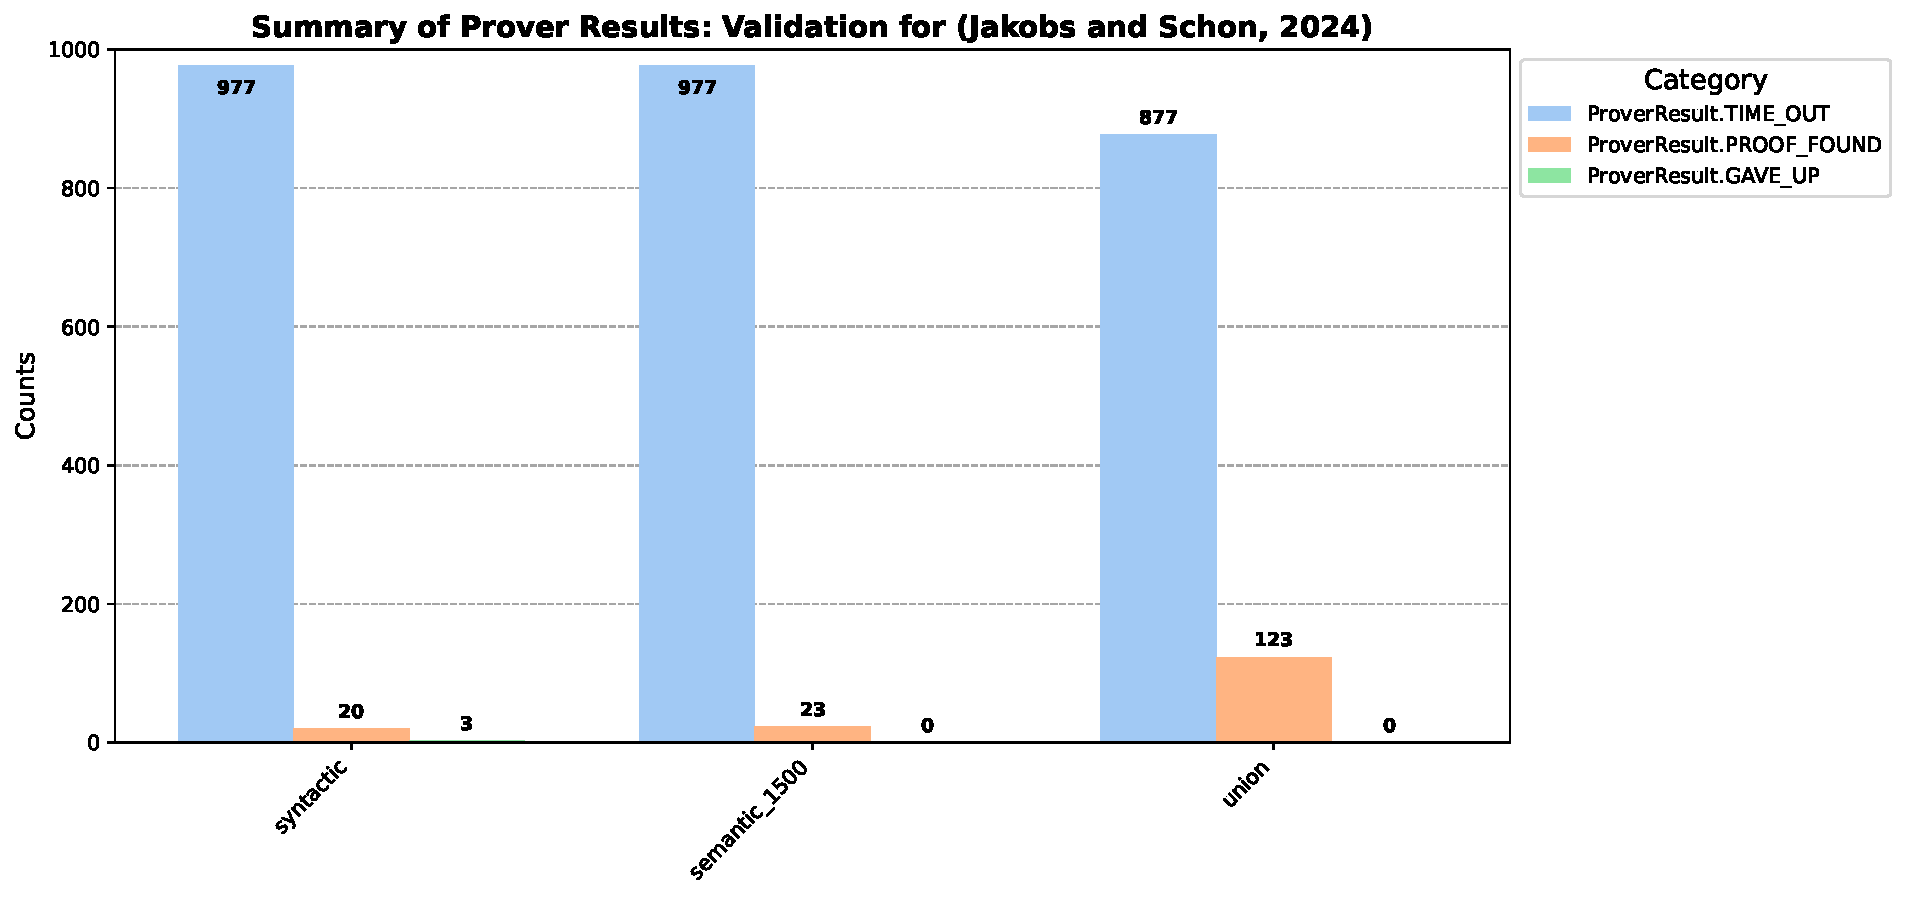
\includegraphics[width=\textwidth]{standard_mode_noAdded_output.pdf}
        \caption{Reengineering of results from \cite{Schon2024}}
        \label{fig:reengineering}
    \end{figure}

    \FloatBarrier

    \item Theorem prover performance is evaluated based on:
    \begin{itemize}
        \item A high percentage of test cases resulted in timeouts or unsuccessful proof attempts, illustrating the difficulty of proving conjectures without additional axioms.
        \item The success rate for proof discovery remained low, suggesting that the standard mode lacks sufficient knowledge for effective inference.
        \item The dataset incorporates multiple axiom selection techniques, including syntactic, semantic-based, and union-based selection.
    \end{itemize}

    \item The distribution of results shows:
    \begin{itemize}
        \item The prover executed 977 test cases, applying each axiom selection approach independently.
        \item The number of successfully proven conjectures was relatively low, reinforcing the importance of improved axiom selection techniques.
        \item Some conjectures had no successful proofs, highlighting weaknesses in current selection strategies.
    \end{itemize}

    \item Implications for further research:
    \begin{itemize}
        \item The findings suggest that semantic similarity alone is insufficient for effective axiom selection.
        \item Further experiments should explore whether the integration of core axioms leads to improved proof success rates.
        \item Analyzing the relationship between axiom complexity and proof success may provide additional insights into theorem proving behavior.
    \end{itemize}
\end{itemize}

\clearpage

\section{Analysis of Reengineering}

The reengineered results are analyzed to better understand proof complexity and selection effectiveness.

\begin{itemize}
    \item The mean variable count in proofs is examined.
    \begin{figure}[h!]
        \centering
        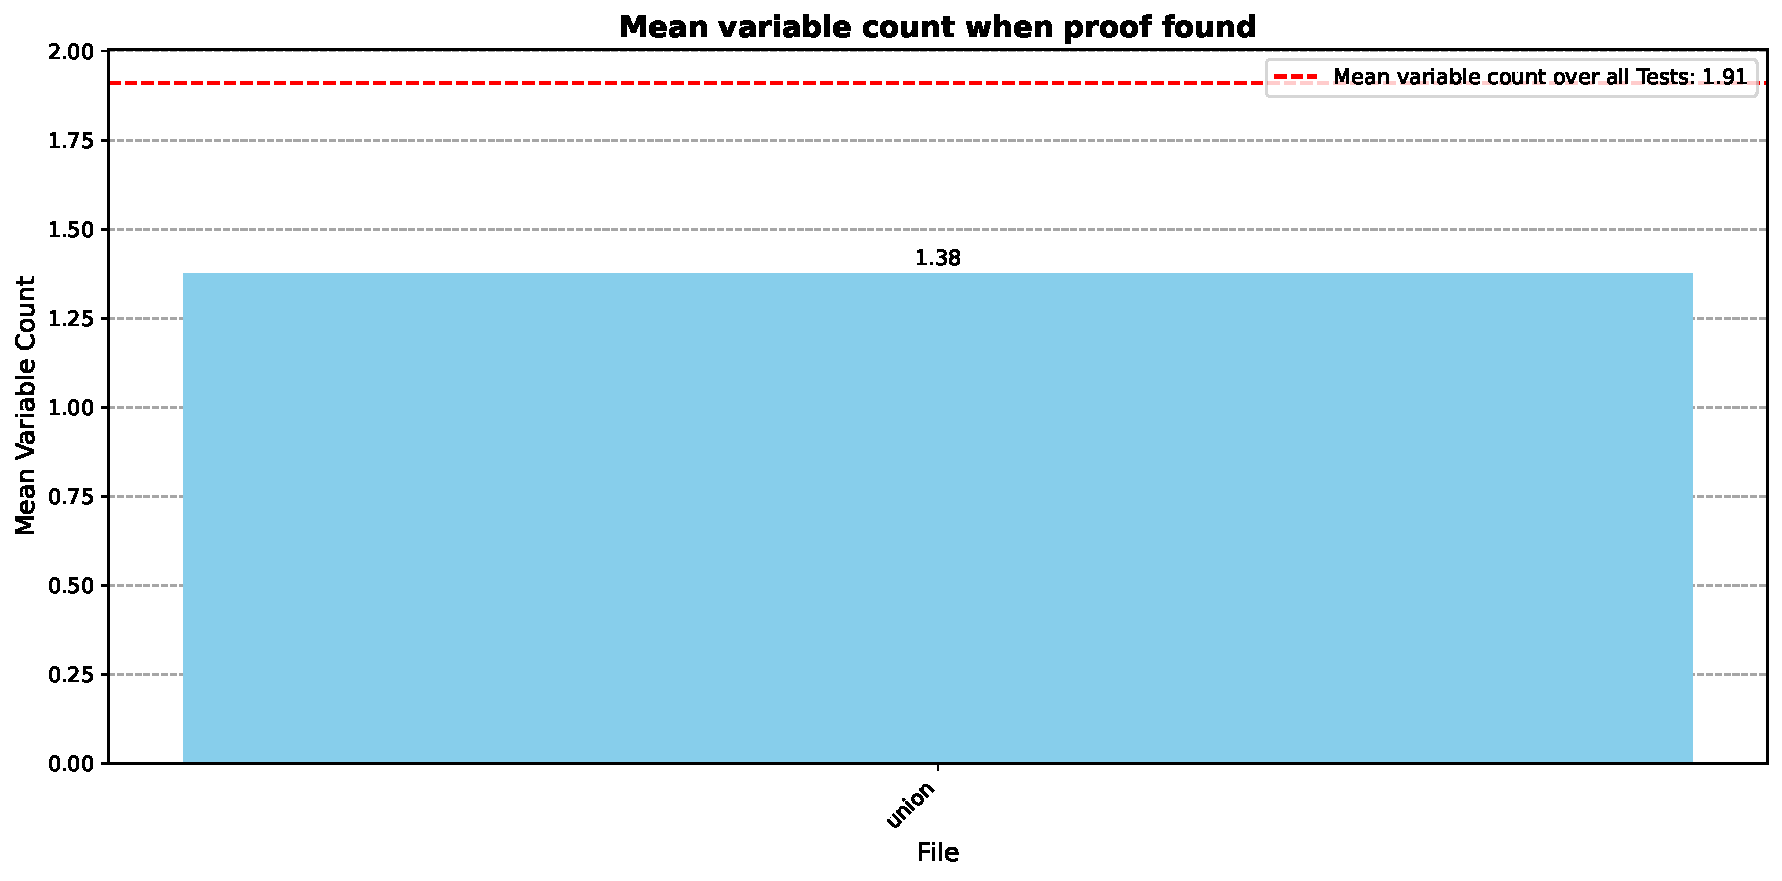
\includegraphics[width=\textwidth]{variable_count_noauto.pdf}
        \caption{Variable count in proofs}
        \label{fig:variable_count}
    \end{figure}
    \FloatBarrier

    \item The count of special symbols in proofs is analyzed.
    \begin{figure}[h!]
        \centering
        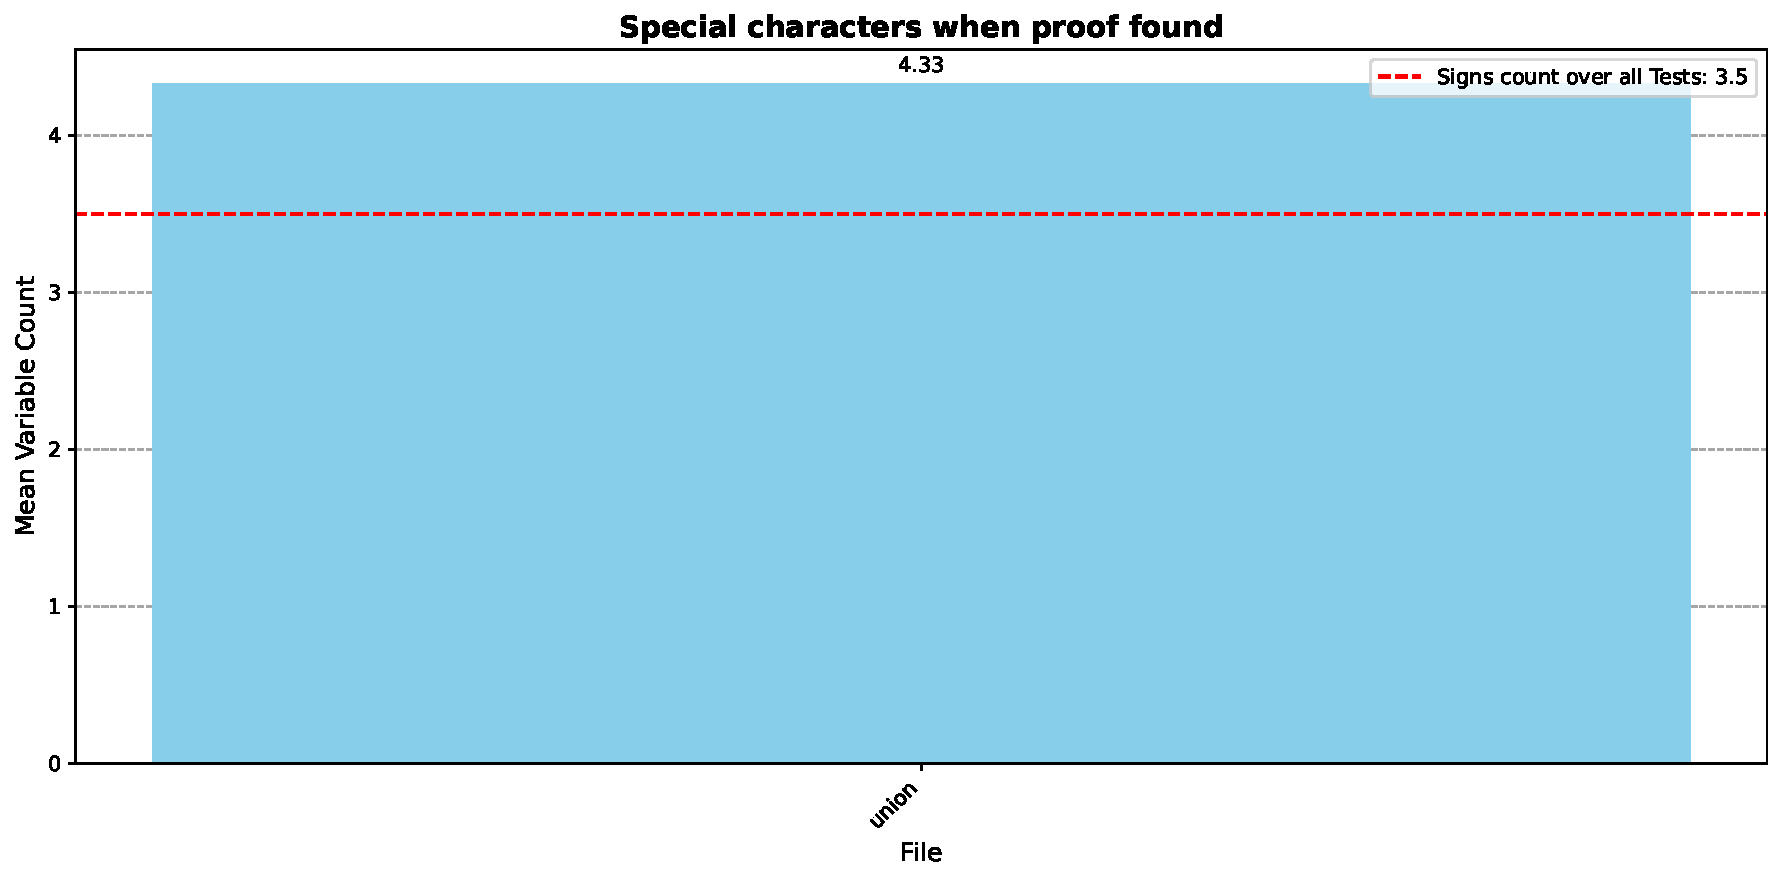
\includegraphics[width=\textwidth]{signs_count_noauto.pdf}
        \caption{Special character count}
        \label{fig:count_signs}
    \end{figure}

    \item The character count across all test cases is examined.
    \begin{figure}[h!]
        \centering
        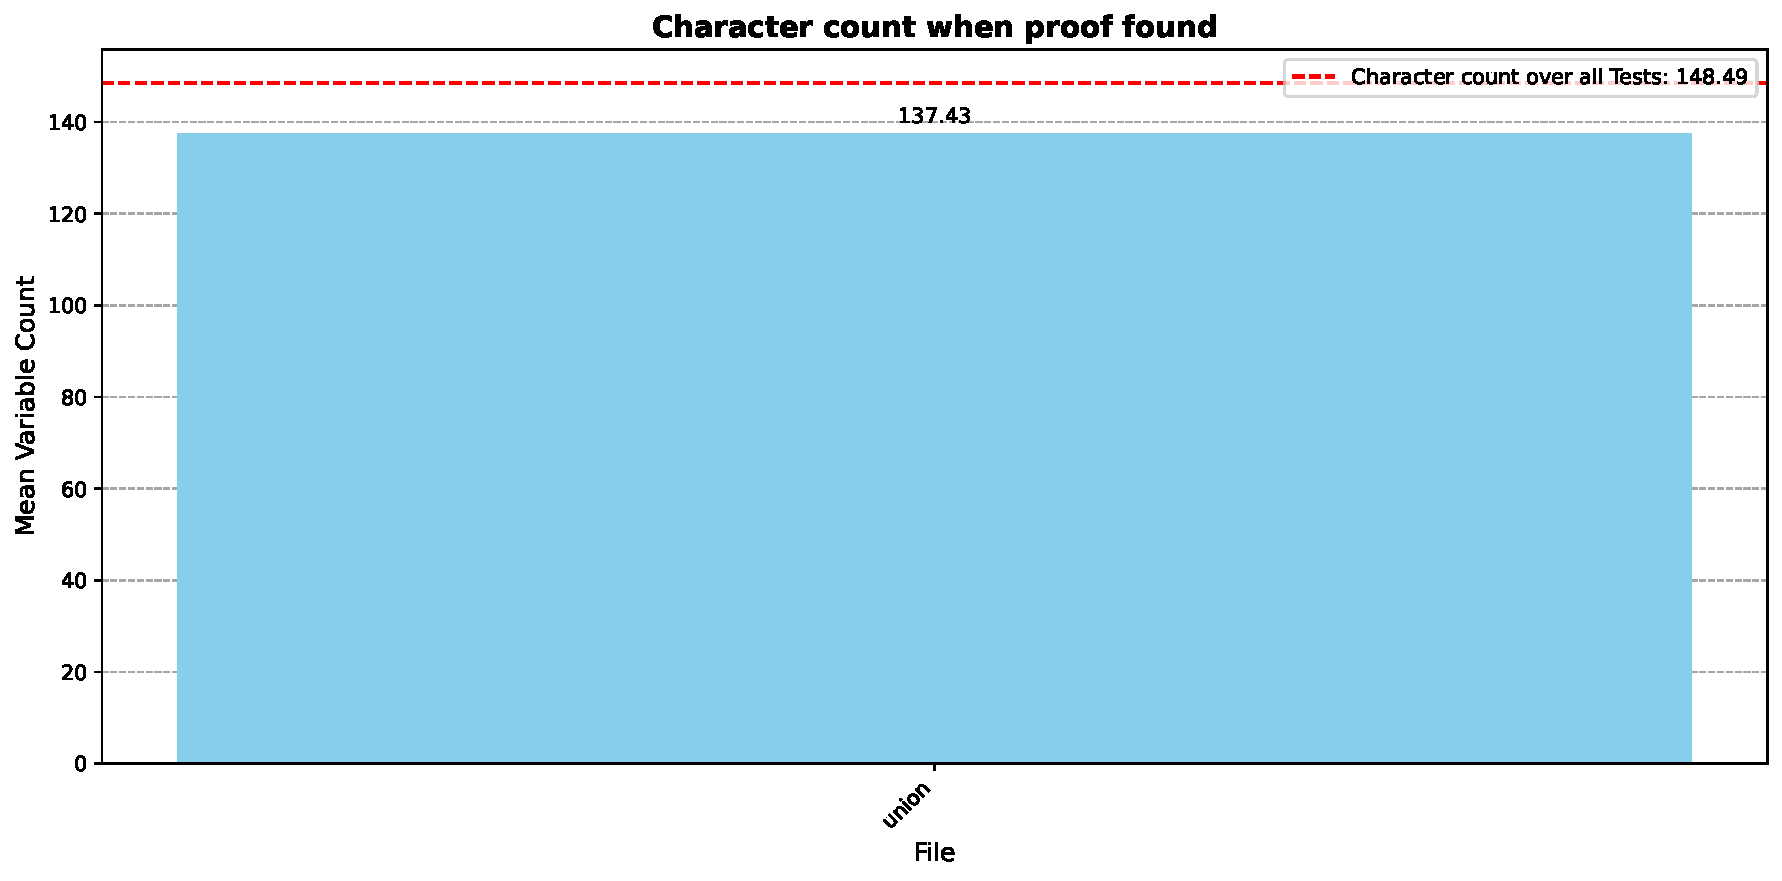
\includegraphics[width=\textwidth]{character_count_noauto.pdf}
        \caption{Character count distribution}
        \label{fig:character_count}
    \end{figure}

    \FloatBarrier

    \item The cosine similarity between axioms and conjectures is analyzed to determine whether similarity influences proof success.
    \begin{figure}[h!]
        \centering
        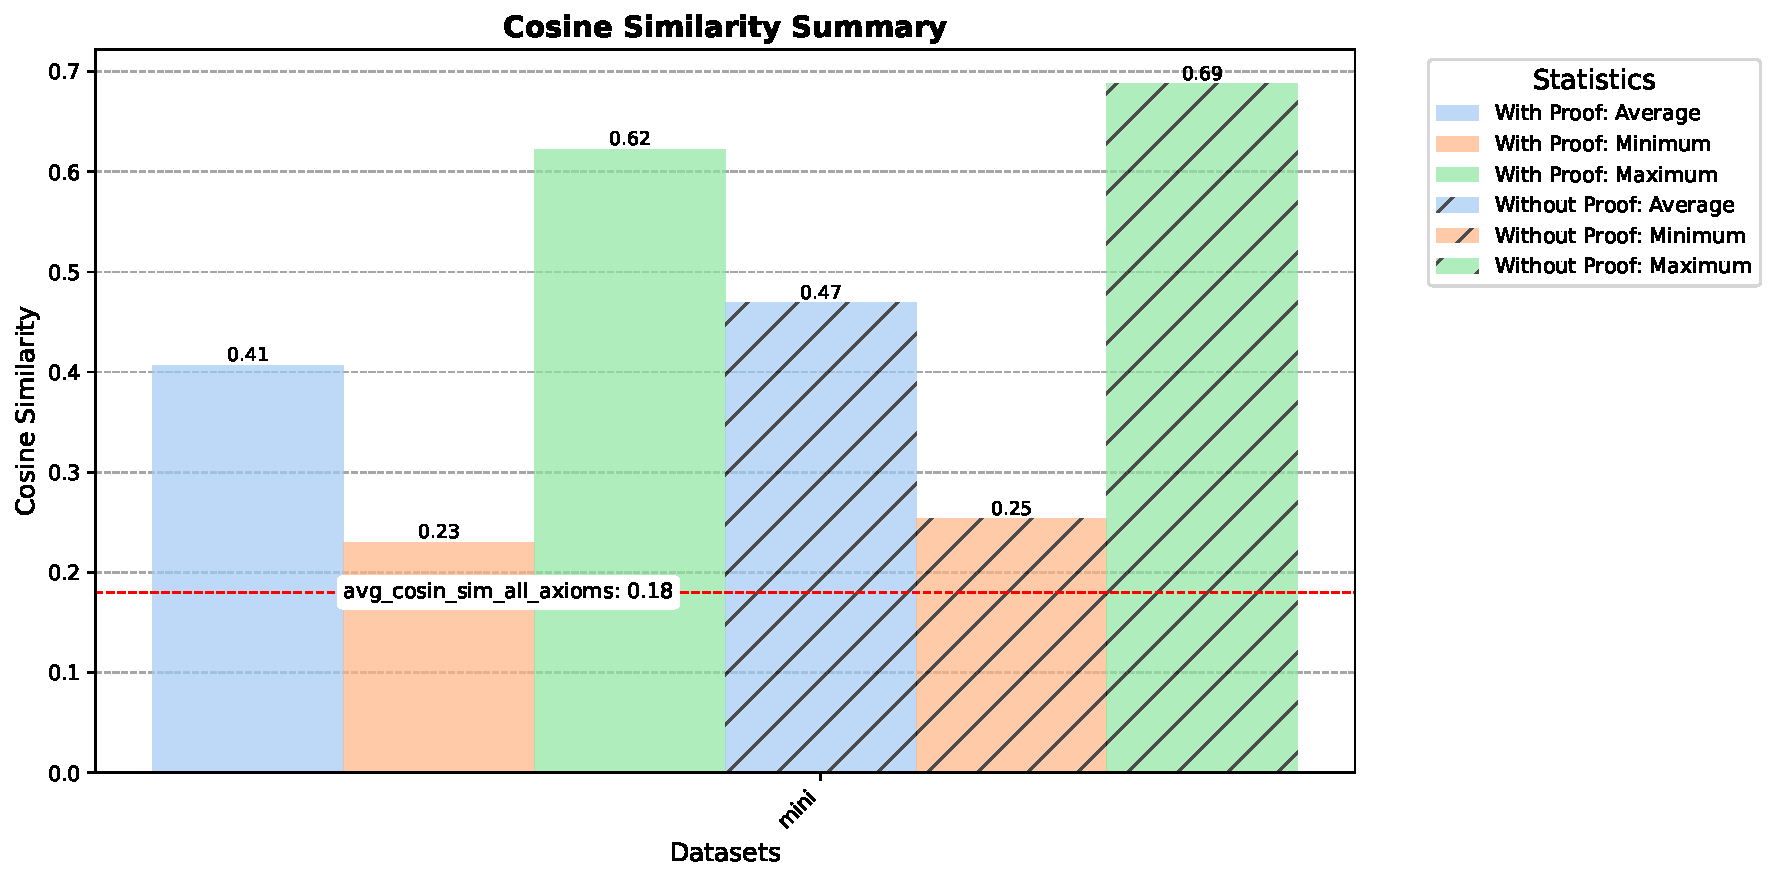
\includegraphics[width=\textwidth]{cosine_similarity_mini_noAdded_summary.pdf}
        \caption{Cosine similarity distribution}
        \label{fig:cosine_similarity}
    \end{figure}
    \FloatBarrier

    The results suggest that provable conjectures often have lower axiom similarity. This indicates that proving a conjecture may require bridging different concepts rather than simply refining closely related axioms.
\end{itemize}

\clearpage

\section{Integration of Core Axioms}

The integration of core axioms into the selection process is evaluated.

\begin{itemize}
    \item The results of theorem proving with core axioms are examined.
    \begin{figure}[h!]
        \centering
        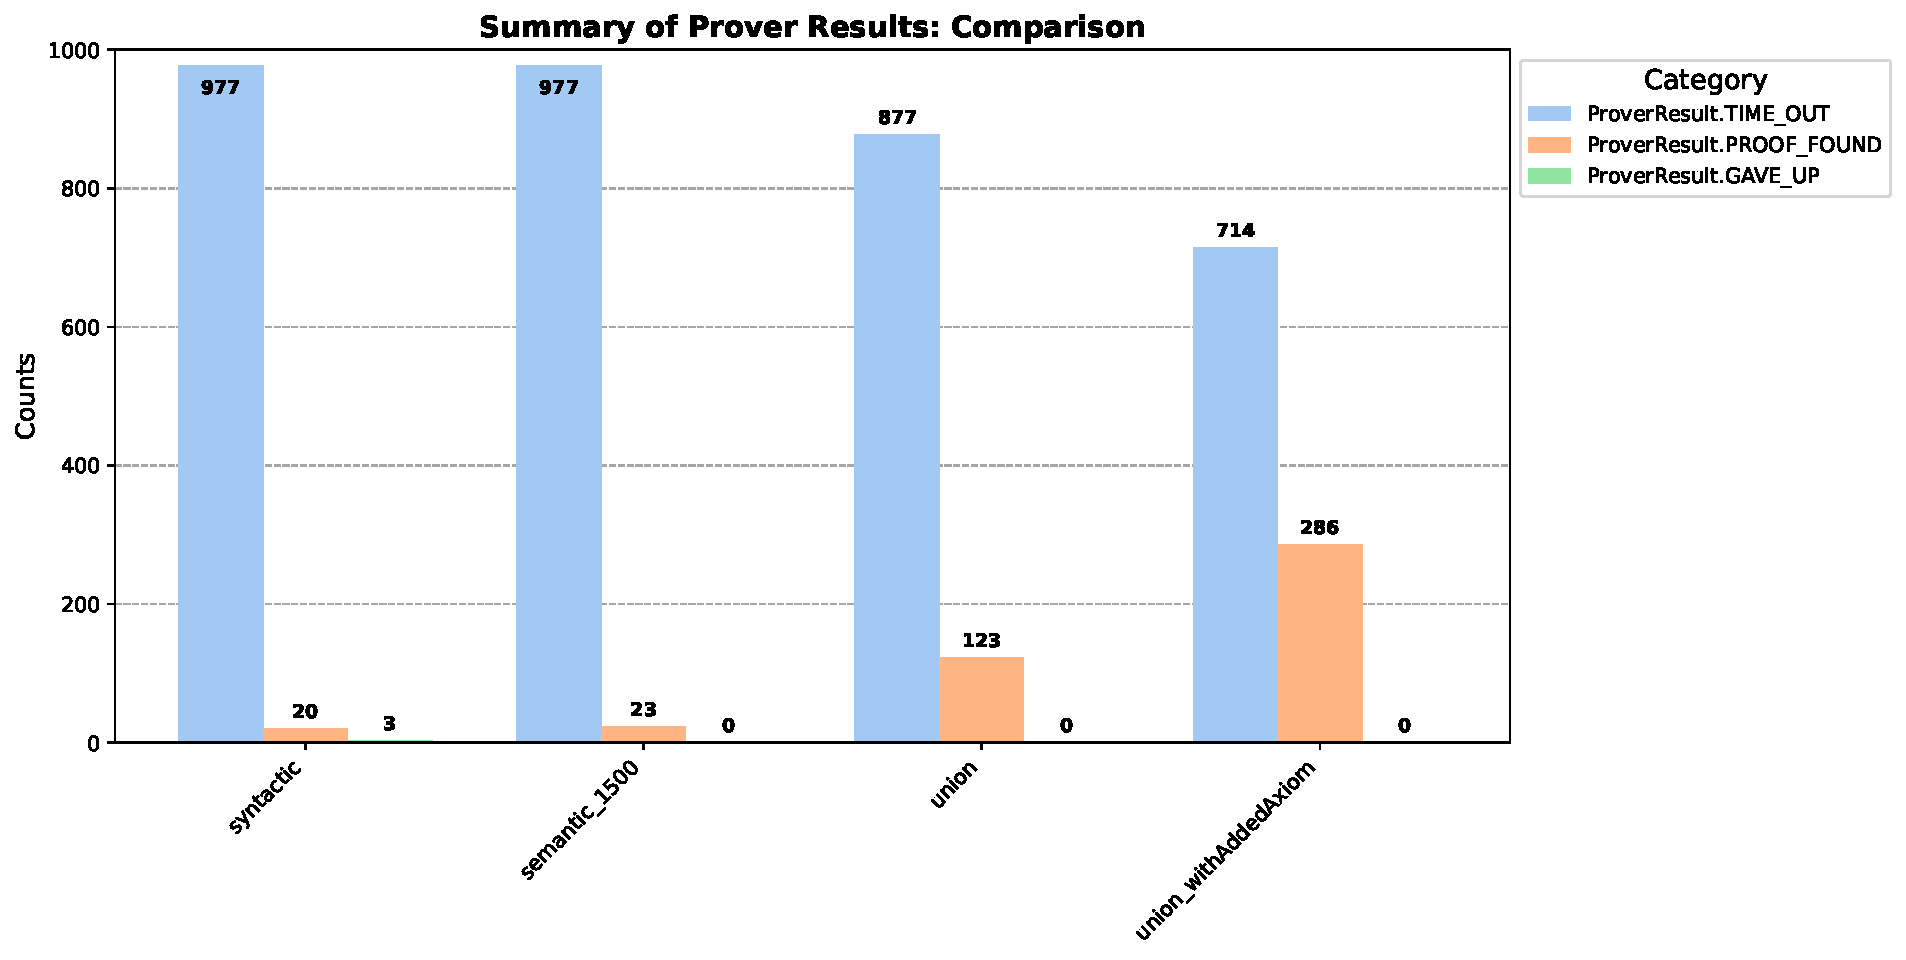
\includegraphics[width=\textwidth]{standard_mode_output.pdf}
        \caption{Summary of prover results with core axioms}
        \label{fig:prover_results_with_core_axioms}
    \end{figure}
    \FloatBarrier

    \item Cosine similarity is compared across different selection methods.
    \begin{figure}[h!]
        \centering
        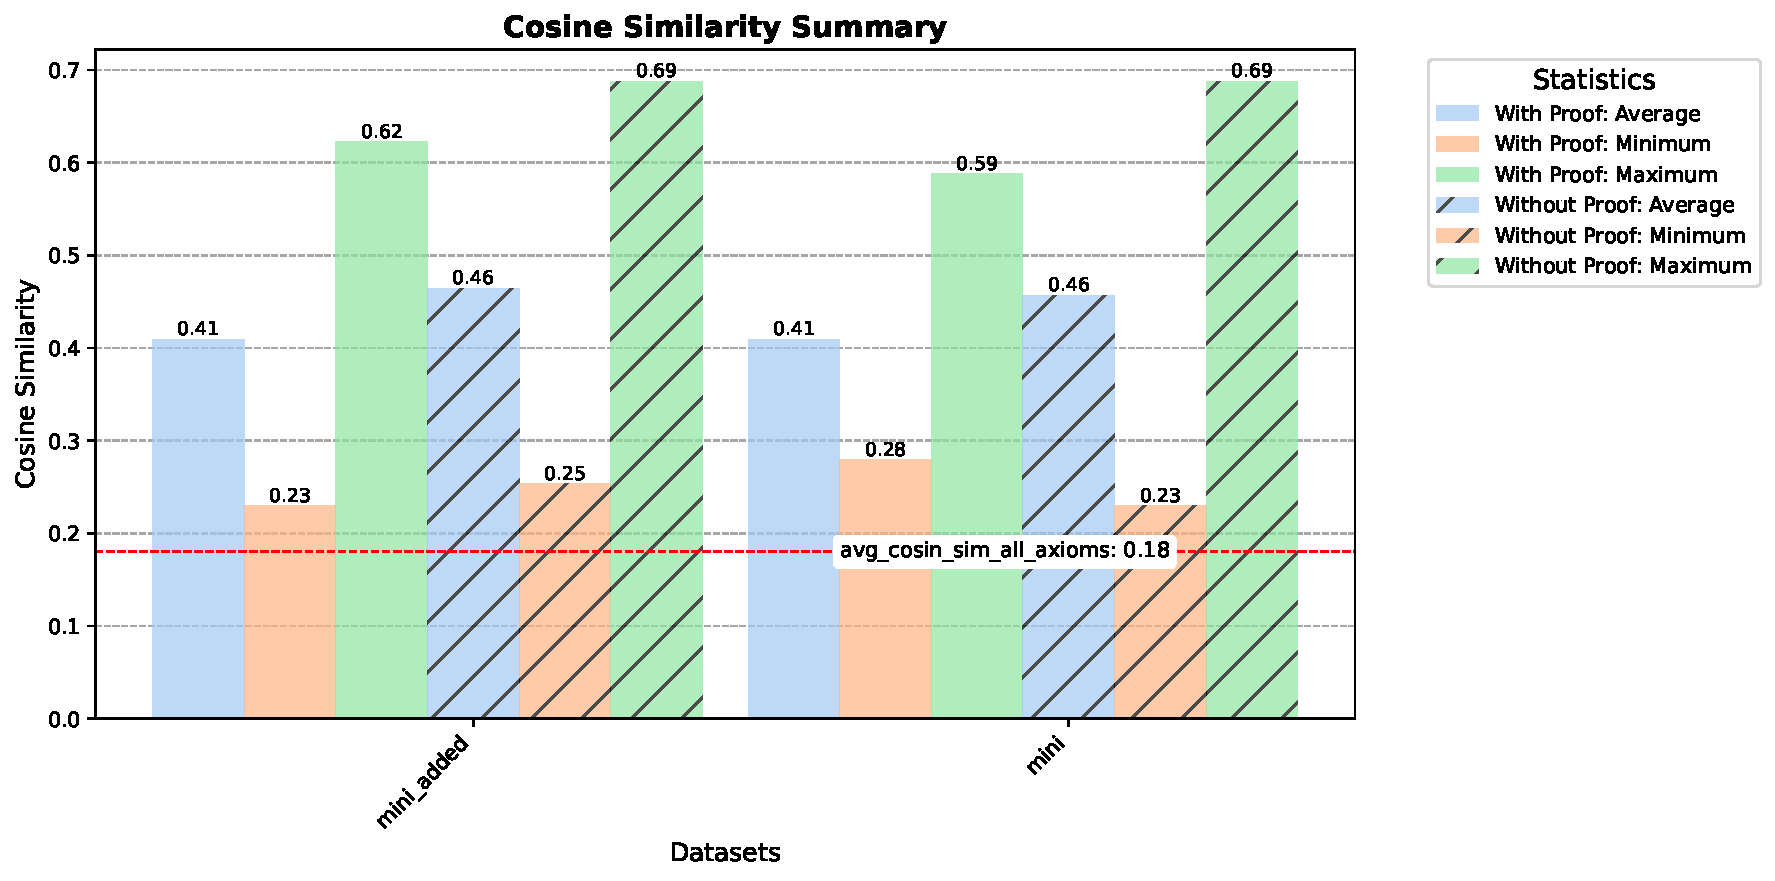
\includegraphics[width=\textwidth]{cosine_similarity_mini_summary.pdf}
        \caption{Cosine similarity comparison}
        \label{fig:prover_results_standard}
    \end{figure}
    \FloatBarrier
\end{itemize}

\clearpage

\section{Comparison of Large Language Models}

The performance of different large language models in axiom selection is assessed.

\begin{itemize}
    \item The results of theorem proving with different models are analyzed.
    \begin{figure}[h!]
        \centering
        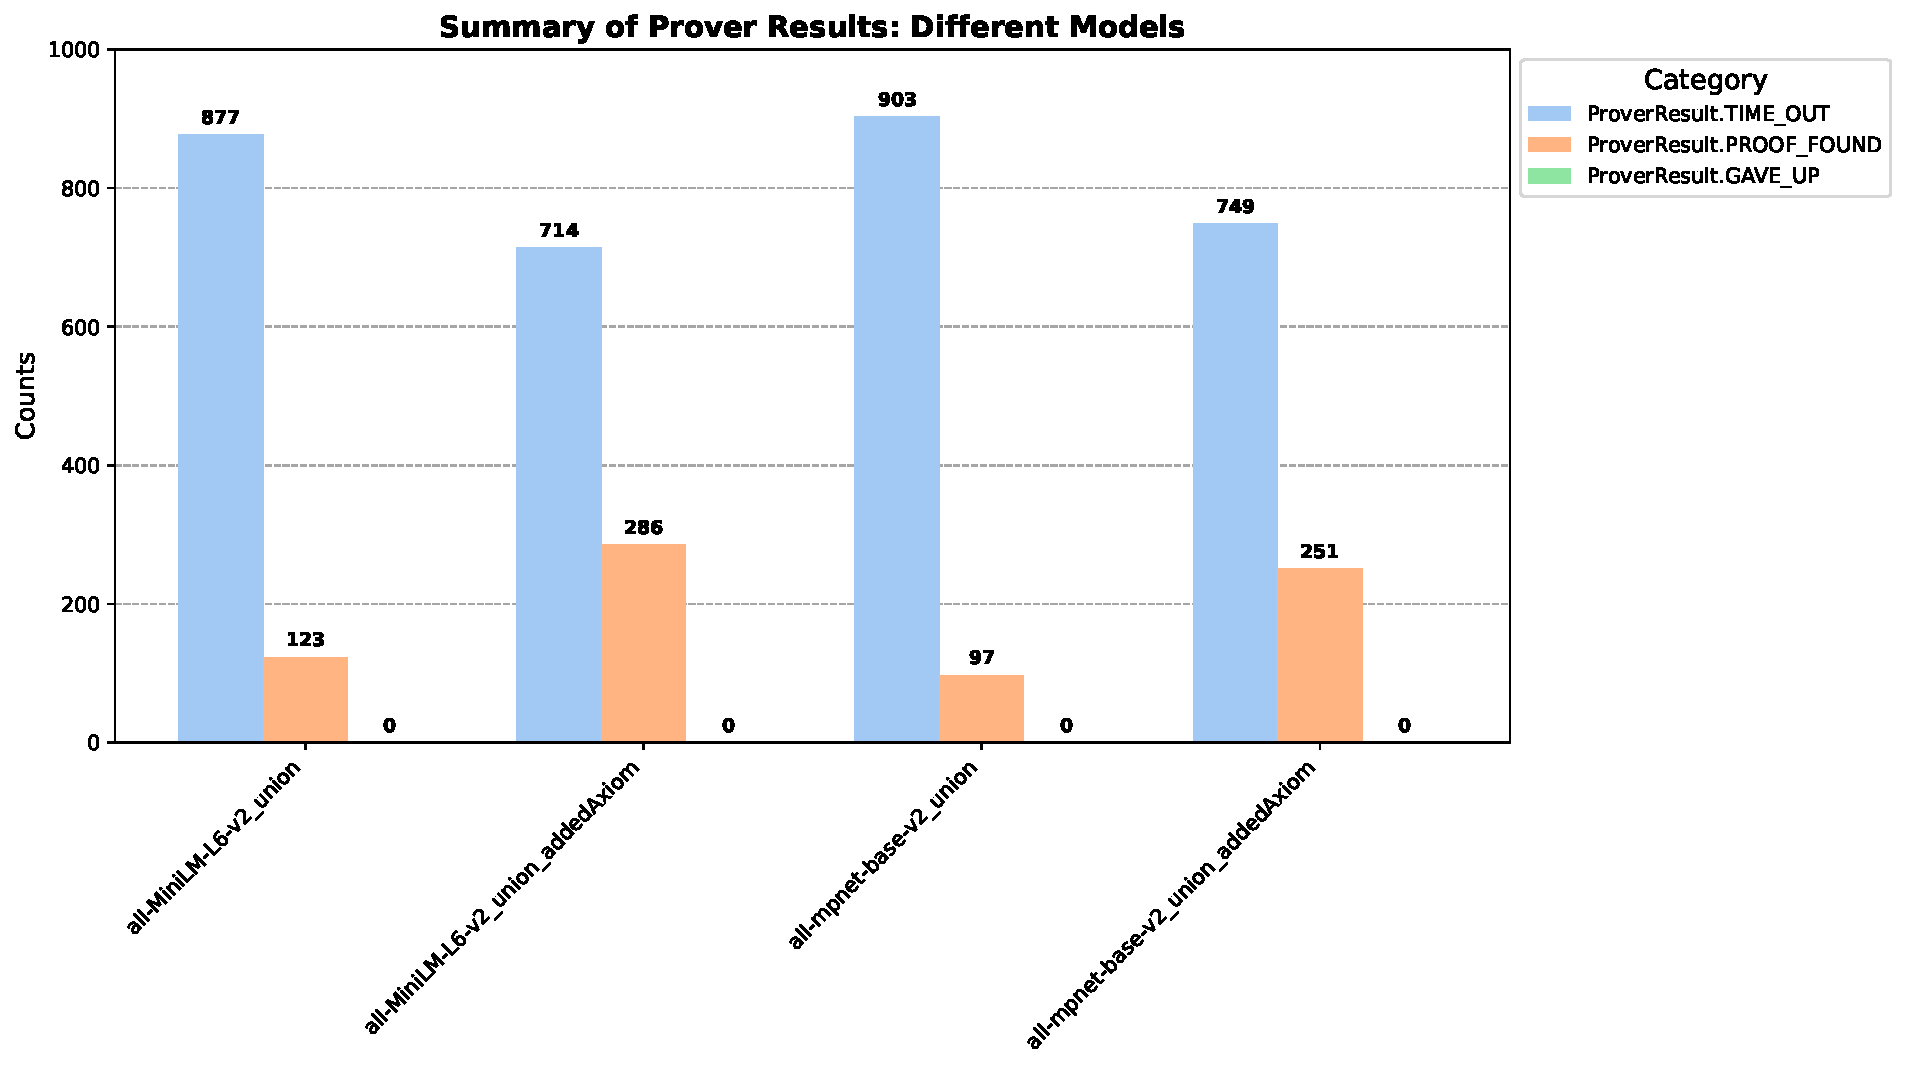
\includegraphics[width=\textwidth]{different_mode_output.pdf}
        \caption{Summary of prover results with different models}
        \label{fig:results_different_models}
    \end{figure}        
    \FloatBarrier

    \item The cosine similarity of selected axioms is compared.
    \begin{figure}[h!]
        \centering
        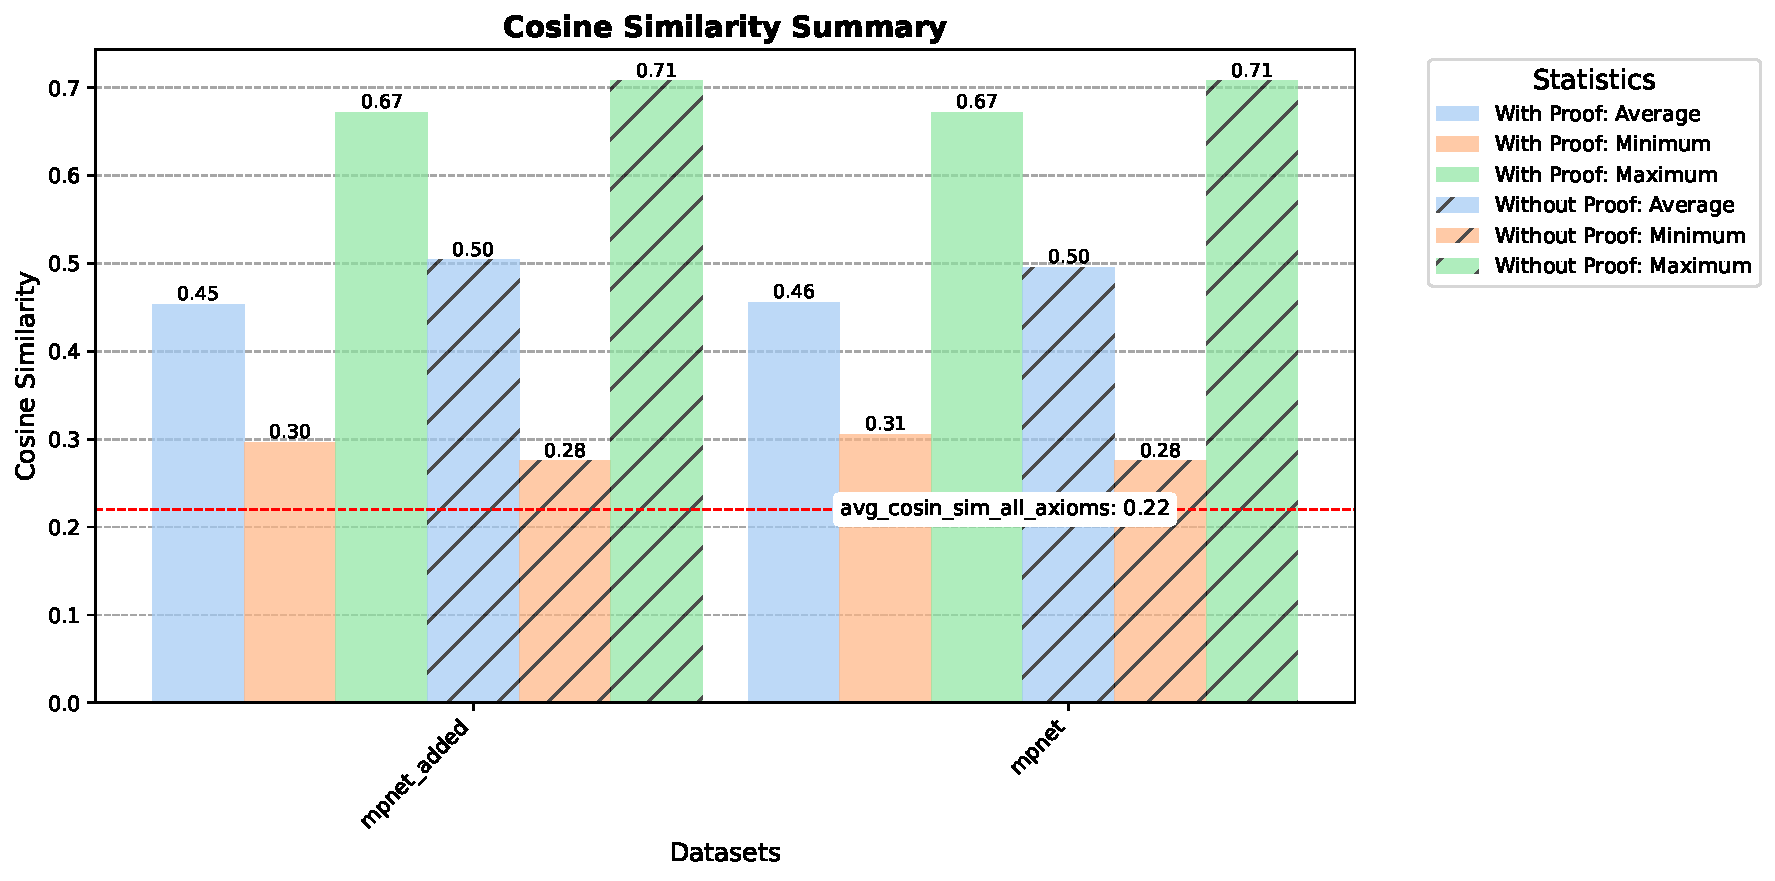
\includegraphics[width=\textwidth]{cosine_similarity_mpnet_summary.pdf}
        \caption{Cosine similarity in different models}
        \label{fig:cosine_similarity_mpnet}
    \end{figure}
    \FloatBarrier
\end{itemize}

\clearpage

\section{Evaluation of Theorem Prover Configurations}

The effect of different theorem prover configurations is analyzed.

\begin{itemize}
    \item The performance of Satauto mode is examined.
    \begin{figure}[h!]
        \centering
        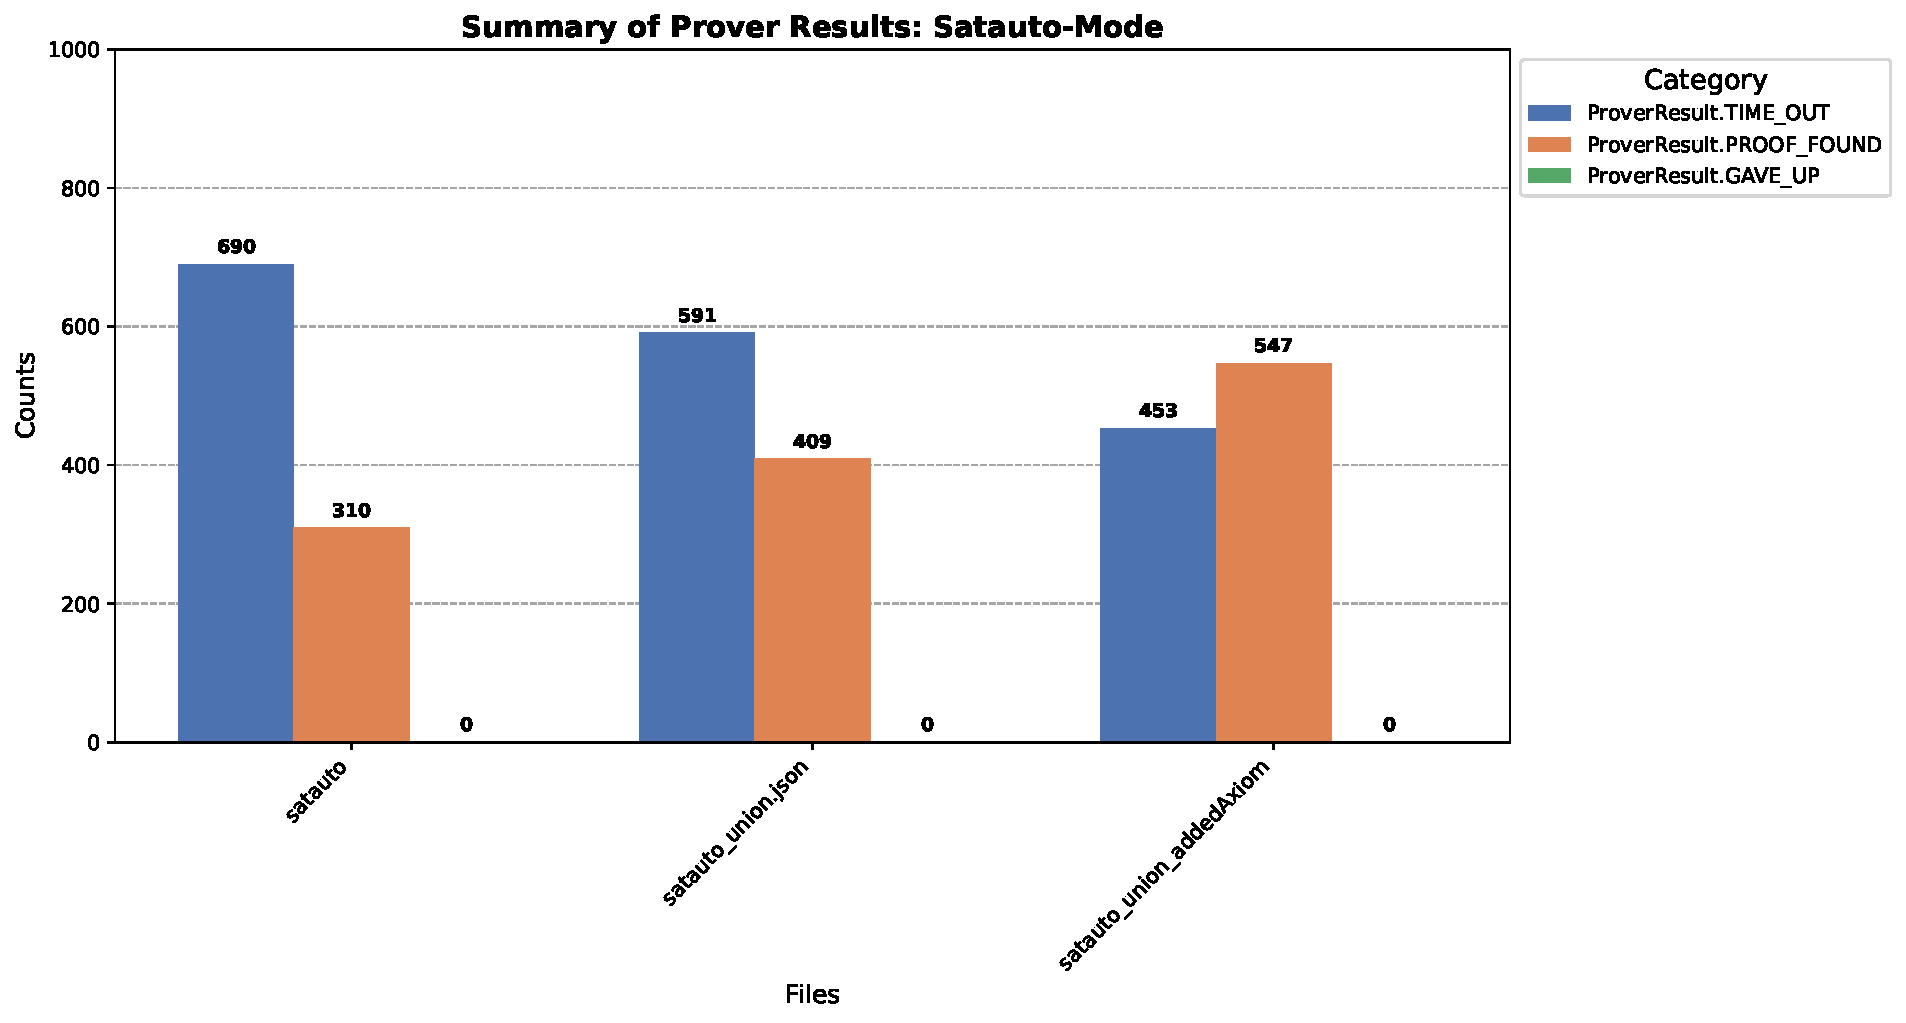
\includegraphics[width=\textwidth]{satauto_mode_output.pdf}
        \caption{Summary of prover results in Satauto mode}
        \label{fig:prover_results_satauto}
    \end{figure}
    \FloatBarrier

    \item The effect of auto mode, which uses SInE and search heuristics, is assessed.
    \begin{figure}[h!]
        \centering
        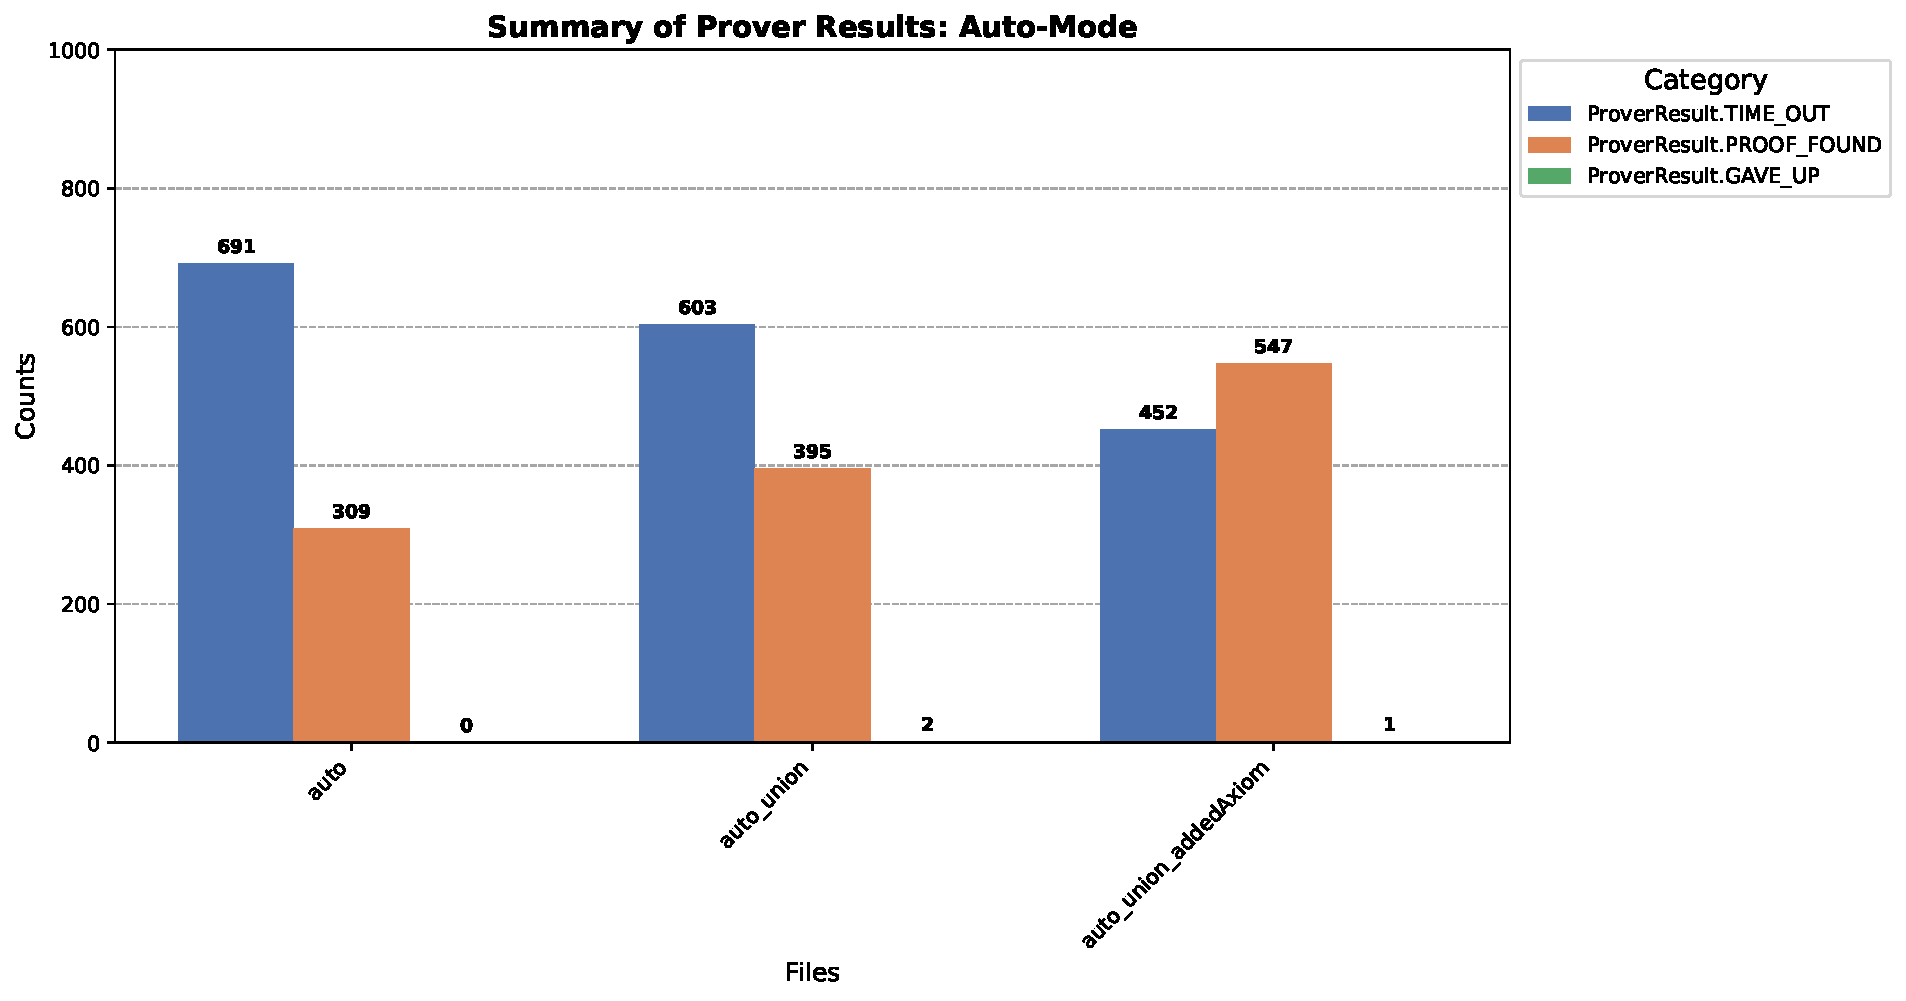
\includegraphics[width=\textwidth]{auto_mode_output.pdf}
        \caption{Summary of prover results in Auto mode}
        \label{fig:prover_results_auto}
    \end{figure}
    \FloatBarrier
\end{itemize}

\clearpage


\chapter{Conclusion}
\label{chapter-conclusion}
Conclusion.
\clearpage

\chapter{Future work}
\label{chapter-futerwork}

Future work.




% Normally, the bibliography comes next at this point. Do *not* (try
% to) include further indices and tables like an index or
% a list of figures or a list of tables or such things. Nobody
% actually uses them and they just use up space. 
%
% You *can* however include a glossary, if this seems appropriate. It
% goes here as an unnumbered chapter. Most thesis will *not* need a
% glossary: a well-written text (re)explains strange words and
% concepts as necessary. However, there are situations where a
% glossary may be helpful.











|$$|


%%%
% 
% Bibliographies
%
%%%
%
% The uzl-thesis class will load biblatex for the bibliography
% management. This is a powerful package, see its documentation for
% details. The styles will be setup correctly and automatically by
% choosing one of the two style keys as described earlier.
%
% In order for the bibliography to work, run latex in the following
% order (which is the standard order):
% 
% > lualatex thesis-example
% > bibtex thesis-example
% > lualatex thesis-example
% 
% Add BibTeX files using \addbibresource or use the {bibtex entries}
% environment (see below).
%
%%%
%
% Although everyting is normally setup automatically, you can change
% the options passed to biblatex using the key 'biblatex';
% for instance,
%
%   \UzLThesisSetup{biblatex={firstinits=false}}
%
% will switch off shortened first names. Normally, you will not need
% this key in your preamble. 
% 
% Note that the bibtex program is used as the 'backend' of biblatex
% by default (rather than biber, which is the preferred program of
% biblatex). This means that you can (and must) run *bibtex* after you
% have run lualatex on your thesis. If you wish to use biber instead
% of bibtex, say 'biblatex={backend=biber}'. 
% 
%%%
%
% The following environment is optional. It allows you to keep the
% bibtex entries for your thesis right here in the thesis file. What
% happens is that each time this tex file is processed, the contents
% of the following environment gets written to the file
% \jobname-bibtex-entries.bib (this file gets overwritten each
% time). Independently, \addbibresource{\jobname-bibtex-entries.bib}
% is always called if the file \jobname-bibtex-entries.bib
% exists. 
%
% In result, you can edit and keep the bibliography's bibtex entries
% right here. If you change something here, run latex, then bibtex,
% then latex once more.
%
% If you would like to manage the bibtex entries in a separate file,
% remove the below environment, delete the \jobname-bibtex-entries.bib
% file and instead write
%
% \addbibresource{filename-of-your-bibtex-file.bib}
%
% in the preamble.
%
%%%


% !!!!!!!!!!!!!!!!!!!!!!!!!!!!!!!!!!
% !!! Your action is needed here !!!
% !!!!!!!!!!!!!!!!!!!!!!!!!!!!!!!!!!
%
% Replace following example entries with the ones of your thesis.

\begin{bibtex-entries}

@InProceedings{Schon2024,
  author="Jakobs, Oliver
  and Schon, Claudia",
  editor="Hotho, Andreas
  and Rudolph, Sebastian",
  title="Context-Specific Selection of Commonsense Knowledge Using Large Language Models",
  booktitle="KI 2024: Advances in Artificial Intelligence",
  year="2024",
  publisher="Springer Nature Switzerland",
  address="Cham",
  pages="218--231",
  abstract="In the field of automated reasoning, practical applications often face a significant challenge: knowledge bases are typically too large to be fully processed by theorem provers. To still be able to prove that a given goal follows from a large knowledge base, selection techniques are used to determine the parts of the knowledge base that are relevant to the goal. Traditional selection techniques used for this task are usually syntax-based and often overlook a crucial aspect---the meaning of symbol names and axioms. Especially in commonsense reasoning scenarios, the meaning embedded in the symbol names provides invaluable insights. For example, in a proof task using the symbol name cow, it intuitively makes more sense to select formulae using the symbol name calf than formulae using the symbol name weapon. To address this gap, our paper introduces a selection technique that exploits the capabilities of large language models. This technique focuses on contextually related formulae, closely aligning the selected part of the knowledge base with the context of the goal. The approach is implemented and we present a series of experiments that show promising results.",
  isbn="978-3-031-70893-0"
}

@article{Àlvez2014,
  author = {Àlvez, Javier and Lucio, Paqui and Rigau, German},
  year = {2014},
  month = {10},
  pages = {80-116},
  title = {Adimen-SUMO: Reengineering an Ontology for First-Order Reasoning},
  volume = {8},
  journal = {International Journal on Semantic Web and Information Systems},
  doi = {10.4018/jswis.2012100105}
}

@InProceedings{Hoder2011,
  author="Hoder, Kry{\v{s}}tof
  and Voronkov, Andrei",
  editor="Bj{\o}rner, Nikolaj
  and Sofronie-Stokkermans, Viorica",
  title="Sine Qua Non for Large Theory Reasoning",
  booktitle="Automated Deduction -- CADE-23",
  year="2011",
  publisher="Springer Berlin Heidelberg",
  address="Berlin, Heidelberg",
  pages="299--314",
  abstract="One possible way to deal with large theories is to have a good selection method for relevant axioms. This is confirmed by the fact that the largest available first-order knowledge base (the Open CYC) contains over 3 million axioms, while answering queries to it usually requires not more than a few dozen axioms. A method for axiom selection has been proposed by the first author in the Sumo INference Engine (SInE) system. SInE has won the large theory division of CASC in 2008. The method turned out to be so successful that the next two years it was used by the winner as well as by several other competing systems. This paper contains the presentation of the method and describes experiments with it in the theorem prover Vampire.",
  isbn="978-3-642-22438-6"
}

@InProceedings{Roederer2009,
  author="Roederer, Alex
  and Puzis, Yury
  and Sutcliffe, Geoff",
  editor="Schmidt, Renate A.",
  title="Divvy: An ATP Meta-system Based on Axiom Relevance Ordering",
  booktitle="Automated Deduction -- CADE-22",
  year="2009",
  publisher="Springer Berlin Heidelberg",
  address="Berlin, Heidelberg",
  pages="157--162",
  abstract="This paper describes two syntactic relevance orderings on the axioms available for proving a given conjecture, and an ATP meta-system that uses the orderings to select axioms to use in proof attempts. The system has been evaluated, and the results show that it is effective.",
  isbn="978-3-642-02959-2"
}

@InProceedings{Sutcliffe2007,
  author="Sutcliffe, Geoff
  and Puzis, Yury",
  editor="Pfenning, Frank",
  title="SRASS - A Semantic Relevance Axiom Selection System",
  booktitle="Automated Deduction -- CADE-21",
  year="2007",
  publisher="Springer Berlin Heidelberg",
  address="Berlin, Heidelberg",
  pages="295--310",
  abstract="This paper describes the design, implementation, and testing of a system for selecting necessary axioms from a large set also containing superfluous axioms, to obtain a proof of a conjecture. The selection is determined by semantics of the axioms and conjecture, ordered heuristically by a syntactic relevance measure. The system is able to solve many problems that cannot be solved alone by the underlying conventional automated reasoning system.",
  isbn="978-3-540-73595-3"
}

@article{Álvez2017,
  author = {Álvez, Javier and Hermo, Montserrat and Lucio, Paqui and Rigau, German},
  year = {2017},
  month = {05},
  pages = {},
  title = {Automatic White-Box Testing of First-Order Logic Ontologies},
  volume = {29},
  journal = {Journal of Logic and Computation},
  doi = {10.1093/logcom/exz001}
}


\end{bibtex-entries}



% If you need to have an appendix (I advise against it), insert it
% here using, first, \appendix and then \chapter and then,
% possibly, \section. 
%
% \appendix
%
% \chapter{Technical Appendix}
%
% \section{Experimental Parameters} % possibly
%
% Again, I advise against using an appendix.


\end{document}

%  LocalWords:  LaTeX tex moretexcs Lübeck pdf uzl lualatex bibtex th
%  LocalWords:  TechReport Kernighan Lamport's Tantau's Tantau cls kZ
%  LocalWords:  Mustermann emacs oldschool pdflatex texmf utf biber
%  LocalWords:  biblatex Alphabetische Bibliographie Numerische VIIa
%  LocalWords:  varioref german Einleitung Beiträge dieser Arbeit xml
%  LocalWords:  Ergebnisse Verwandte Arbeiten Aufbau nucleotide VIIc
%  LocalWords:  ensembl amino phylogenetic Alexa Siri decrypt versa
%  LocalWords:  cryptographic pre nondeterministic deterministically
%  LocalWords:  Beutelspacher Untersuchungen zum genetischen sep llcc
%  LocalWords:  Beispiel tikz jpg png Alegrya Kasimir Malewitsch PGF
%  LocalWords:  Lamport Institut für Theoretische Informatik zu url
%  LocalWords:  Universität Springer DowneyF Downey Parameterized doi
%  LocalWords:  BibLaTeX Kime Philipp urldate Mittelbach hyperref Lua
%  LocalWords:  Rahtz Oberdiek Heiko Braams Bezos López fontspec Das
%  LocalWords:  Arseneau amsmath ist Tipps und zur Formulierung
%  LocalWords:  mathematischer Gedanken Mathematik Studienanfänger
%  LocalWords:  Albrecht Vieweg Teubner Verlag
